\documentclass[11pt, oneside]{article}   	% use "amsart" instead of "article" for AMSLaTeX format
\usepackage{geometry}                		% See geometry.pdf to learn the layout options. There are lots.
\geometry{letterpaper}                   		% ... or a4paper or a5paper or ... 
%\geometry{landscape}                		% Activate for for rotated page geometry
%\usepackage[parfill]{parskip}    		% Activate to begin paragraphs with an empty line rather than an indent
\usepackage{graphicx}				% Use pdf, png, jpg, or eps§ with pdflatex; use eps in DVI mode
								% TeX will automatically convert eps --> pdf in pdflatex		
\usepackage{amssymb}
\usepackage{amsmath}
\usepackage{parskip}
\usepackage{color}
\usepackage{hyperref}

\title{Sum and product rule}
%\author{The Author}
%\section{}
%\subsection*{}
\date{}							% Activate to display a given date or no date

\graphicspath{{/Users/telliott_admin/Dropbox/Tex/png/}}
% \begin{center} 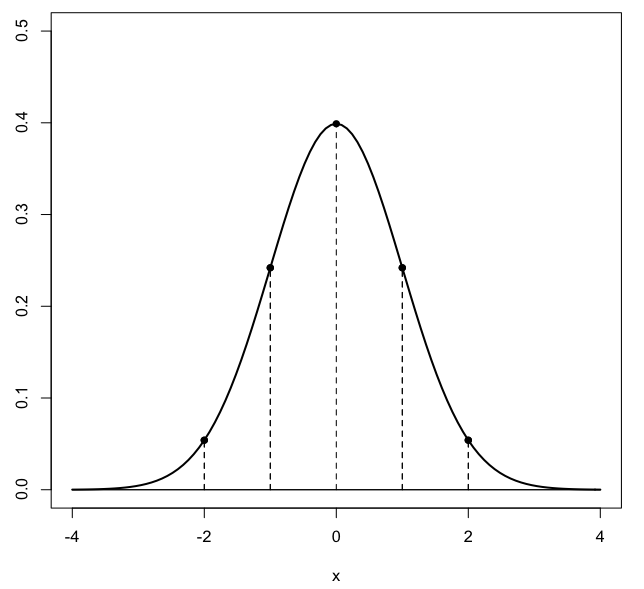
\includegraphics [scale=0.4] {gauss3.png} \end{center}
\begin{document}
\maketitle
\Large

Assume that
\[ \lim_{x \rightarrow c} f(x) = L \]
\[ \lim_{x \rightarrow c} g(x) = M \]

We want to show that
\[ \lim_{x \rightarrow c} f(x) + g(x) = L + M \]
The limit of the sum is the sum of the limits.

Let $\epsilon > 0$ be arbitrary.

Then the existence of the limits means that
\[ \forall \ \epsilon, \exists \ \delta_1 > 0 \ | \ \forall \ x, \ 0 < | x - c| < \delta_1 \rightarrow | f(x) - L | < \epsilon/2 \]
and
\[ \forall \ \epsilon, \exists \ \delta_2 > 0 \ | \ \forall \ x, \ 0 < | x - c| < \delta_2 \rightarrow | g(x) - M | < \epsilon/2 \]
Let
\[ \delta = \text{ min } (\delta_1, \delta_2) \]
Now for $|x - c| < \delta$:
\[ | f(x) - L + g(x) - M| < \epsilon \]
But by the triangle inequality the left-hand side is 
\[   | f(x) - L| + |g(x) - M| < \epsilon \]
which proves the theorem.

\subsection*{proof of the product rule for limits}
Assume that
\[ \lim_{x \rightarrow c} f(x) = L \]
\[ \lim_{x \rightarrow c} g(x) = M \]

We want to show that
\[ \lim_{x \rightarrow c} f(x) \cdot g(x) = LM \]
The limit of the product is the product of the limits.

We need to show that
\[ f(x) \cdot g(x) - LM \]
is small.  

Subtract $L g(x)$ and add it back
\[ f(x) \cdot g(x) - LM = f(x) \cdot g(x) - L g(x) + L g(x) - LM \]
\[ = (f(x) - L) g(x) + L (g(x) - M ) \]
Take the absolute value on both sides
\[  |f(x) \cdot g(x) - LM| = |(f(x) - L) \cdot g(x) + L \cdot (g(x) - M )| \]
Use the triangle inequality to split up the sum:
\[ \le |(f(x) - L) \cdot g(x)| + |L \cdot (g(x) - M )| \]
This can be further massaged to 
\[  =| f(x) - L | \cdot |g(x)| + |L| \cdot |g(x) - M | \]
Write the whole thing:
\[ |f(x) \cdot g(x) - LM| \le |(f(x) - L) | | g(x) | + | L | | (g(x) - M )| \]

Now, play the epsilon-delta game:  you pick $\epsilon$ and then I concentrate on a region so close to $c$ that
\[ |f(x) - L | < \epsilon \]
and
\[ |g(x) - M | < \epsilon \]

If your epsilon is too large it would mess things up (why?), so in that case I will pick $|g(x) - M| = 1$.

Then I have
\[ |f(x) - L | < \epsilon \]
\[ |g(x) - M | < \epsilon \]
\[ |g(x)| < |M| + 1 \]

Go back to the equation we obtained above
\[ |f(x) \cdot g(x) - LM| \le |(f(x) - L) | | g(x)| + | L | | (g(x) - M )| \]
substitute on the right-hand side
\[ |(f(x) - L) | | g(x)| + | L | | (g(x) - M )| \]
\[ \le \epsilon \ (|M| + 1) + | L | \ \epsilon \]
\[ \le \epsilon \ (|M| + |L| + 1) \]
That is:
\[ |f(x) \cdot g(x) - LM| \le \epsilon \ (|M| + |L| + 1) \]

as Adrian Banner says in \emph{Calculus Lifesaver}:

\begin{quote}
That's almost what I want!  I was supposed to get $\epsilon$ on the right-hand side, but I got an extra factor of $|M| + |L| + 1$.  This is no problem---you just have to allow me to make my move again, but this time I'll make sure that $|f(x) - L|$ is no more than $\epsilon/2(|M| + |L| + 1)$, and similarly for $|g(x) - M|$.  Then when I replay all the steps, $\epsilon$ will be replaced by $\epsilon/(|M| + |L| + 1)$, and at the very last step, the factor $|M| + |L| + 1$ will cancel out and we'll just get our $\epsilon$.  So we have proved the result.
\end{quote}

\subsection*{More formal proof of the product rule}

Suppose that 
\[ \lim_{x \rightarrow c} f(x) = L \]
\[ \lim_{x \rightarrow c} g(x) = M \]

To prove:
\[ \lim_{x \rightarrow c} f(x) \cdot g(x) = LM \]

\subsection*{Proof}
Let $\epsilon > 0$.  By the definition of limits we can find three numbers $\delta_1$, $\delta_2$ and $\delta_3$ such that

if $0 < |x - c| < \delta_1$:
\[ |f(x) - L| < \frac{\epsilon}{2(1 + |M|)} \]
if $0 < |x - c| < \delta_2$:
\[ |g(x) - M| < \frac{\epsilon}{2(1 + |L|)} \]
and third, if $0 < |x - c| < \delta_3$:
\[ |g(x) - M| < 1 \]

Now write
\[ |g(x)| = |g(x) - M + M| \]
use the triangle inequality
\[ |g(x)| \le |g(x) - M| + |M|\]
Then according to (3), if if $0 < |x - c| < \delta_3$:
\[ |g(x) \le 1 + |M|  \]

Choose $\delta = \min \{\delta_1,\delta_2,\delta_3\}$.

Then if $0 < |x - c| < \delta$:
\[ |f(x) \cdot g(x) - LM| = |f(x) \cdot g(x) - L \cdot g(x) + L \cdot g(x) - LM| \]
by the triangle inequality (again)
\[ \le |f(x) \cdot g(x) - L \cdot g(x)| + |L \cdot g(x) - LM| \]
The next step is to factor (see below):
\[ \le |g(x)| |f(x) - L| + |L| |g(x) - M| \]
\[ < (1 + |M|) \ \frac{\epsilon}{2(1 + |M|)} + (1 + |L|) \ \frac{\epsilon}{2(1 + |L|)} \]
\[ < \frac{\epsilon}{2} + \frac{\epsilon}{2} \]
\[ |f(x) \cdot g(x) - LM| < \epsilon \]
which completes the proof.

\end{document}  